%!TEX TS-program = pdflatex
%!TEX root = progetto_finale.tex
%!TEX encoding = UTF-8 Unicode

\chapter{Progetto} \label{progetto}

In questo capitolo vengono descritte l'architettura del software, i protocolli e gli algoritmi utilizzati, l'architettura fisica e il piano di sviluppo.

\section{Architettura Logica}

Qui di seguito sono descritti i vari moduli che si intende implementare per il progetto:

\begin{itemize} \label{modules}
	\item Modulo Entità Utente: rappresenta l'astrazione dell'entità utente.
	\item Modulo Entità Ambiente : rappresenta l'astrazione dell'entità ambiente.
	\item Mappa Città: fornisce i metodi di lettura e modifica della mappa della città. Per le modifiche utilizza il modulo degli algoritmi sui grafi per controllarne la fattibilità. Questo modulo astrae il fatto che è presente un grafo per la rappresentazione della mappa.
	\item Algoritmi Grafo: fornisce gli algoritmi che è possibile utilizzare sui grafi. Per esempio include Dijkstra, BFS, DFS, aggiungi nodo / arco, ...
	\item Localizzatore Vicini: permette di conoscere le entità vicine.
	\item Invio Messaggi: permette la comunicazione fra entità controllando la buona formattazione dei messaggi da inviare. Essa simula la scheda di comunicazione.
	\item Modulo Taxi: è formato al suo interno da due moduli:
	\begin{itemize}
		\item Modulo per l'algoritmo di elezione del leader: implementa la funzionalità della scelta della macchina da assegnare all'utente.
		\item Modulo gestione taxi: esso è l'interfaccia con cui l'applicazione dell'utente comunica con un determinato taxi. Fornisce i metodi di prenotazione di una corsa, gestisce gli eventi generati dal sistema, fornisce il servizio di spostamento.
	\end{itemize}
	\item Modulo interfaccia cliente-servizio: rappresenta l'applicazione che utilizzerebbe l'utente per usufruire del servizio. In tal senso, fornisce le operazioni che un cliente può richiedere al sistema e comunica ad egli gli eventuali messaggi. Il modulo di gestione del taxi comunica a questo modulo gli eventuali cambi di stato.
	\item Modulo gestione tempo: simula un orologio utilizzato per la gestione degli spostamenti e timeout.
\end{itemize}

Le relazioni e le dipendenze tra di essi sono presenti all'immagine \ref{fig:schema_moduli_livello_0}. Le immagini \ref{fig:schema_moduli_livello_1} e \ref{fig:schema_moduli_livello_2} ne approfondiscono il significato.

In questi schemi le bolle rappresentano i suddetti moduli: sono colorate di rosso per gli attori, ossia i moduli principali, e di verde per i fornitori di funzionalità, ossia i moduli secondari. La bolla ``clock'' indica il modulo gestione tempo ed è stata colorata in azzurro  poiché non fornisce nessun'altra funzionalità al di là del comunicare lo scorrere del tempo.  

Gli archi indicano una relazione di dipendenza con questa semantica: un arco che parte da una bolla A e arriva in una bolla B indica che A conosce B e che vi comunica. Si noti che la relazione non è simmetrica. Nel caso di relazione tra un attore e un fornitore di funzionalità, la comunicazione si intende come ``utilizzo dei servizi offerti'', mentre nel caso della relazione attore-attore si intende ``effettua scambi di messaggi''.

\begin{figure}[htbp]
	\centering
	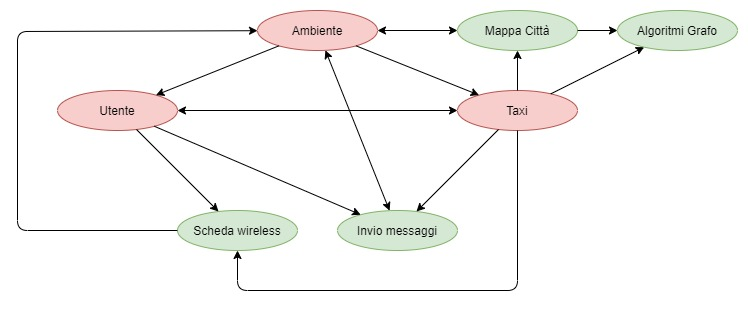
\includegraphics[width=15cm]{schema_moduli_livello_0.jpg}
	\caption{Dipendenze tra i moduli livello 0}
	\label{fig:schema_moduli_livello_0}
\end{figure}


L'immagine \ref{fig:schema_moduli_livello_1} specializza le relazioni precedentemente definite incorporando i restanti moduli. In giallo sono state colorate le bolle che specializzano le entità Utente e Taxi.

\begin{figure}[htbp]
	\centering
	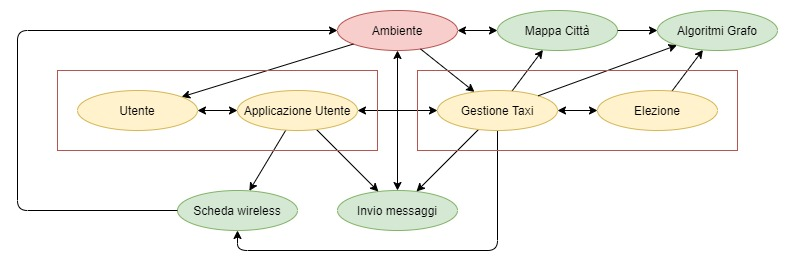
\includegraphics[width=15cm]{schema_moduli_livello_1.jpg}
	\caption{Dipendenze tra i moduli livello 1}
	\label{fig:schema_moduli_livello_1}
\end{figure}

\newpage

\section{Automi Coinvolti} \label{automi}

Per rappresentare il comportamento delle entità coinvolte in base ai possibili eventi, sono stati creati diversi automi che codificano i possibili stati delle macchine e degli utenti. 
Si è deciso di suddividere le suddette entità in più automi, ognuno di questi dedicato a una funzione specifica. 
In particolare, l'utente è stato modellato con:
\begin{itemize} 
 \item automa\_utente : la rappresentazione dell'utente e di tutti gli eventi che possono interessargli.
 \item automa\_app\_utente : la rappresentazione dell'utente dal punto di vista del servizio. Questo automa è l'istanza del servizio per un particolare utente, l'automa\_utente comunica con questo per poter usare il servizio così come i taxi o il servizio stesso per poter comunicare con l'automa\_utente.
\end{itemize}

Il Taxi è stato invece modellato con questi automi:
\begin{itemize} 
 \item automa\_moving: rappresenta il veicolo in servizio.
 \item automa\_elezione: descrive gli stati per l'algoritmo di elezione ed eventi associati. 
 \item automa\_batteria: rappresenta un sensore della batteria interna al veicolo, notificando, quando necessario, che è necessario ricaricarla oppure lo stato di fermo della macchina per un certo periodo di tempo.
 \item automa\_listener: ascoltatore dei possibili eventi che interessano al veicolo. Riceve messaggi dall'ambiente, comunica con l'automa dell'applicazione dell'utente e con gli automi suoi pari negli altri veicoli. Esso è anche il tramite verso gli automi interni al veicolo: ogni evento indirizzato ad essi viene prima catturato da questo automa e poi inviato al corretto destinatario. Nel caso in cui riceve un messaggio di inizio elezione, questo automa si sposta nello stato ``listen\_election''. Questo speciale stato comporta che vengano considerati solo i messaggi relativi all'elezione, tutti gli altri vengono messi in una speciale coda e verranno gestiti alla fine dell'elezione.
\end{itemize} 

All'interno del servizio, quando viene creato un nuovo utente oppure un nuovo taxi, vengono generate istanze di ogni automa correlato, vale a dire, quindi, i due automi per l'utente e i quattro automi per il taxi. Nel momento in cui un cliente è stato servito portandolo a destinazione, oppure un taxi viene rimosso dalla mappa, vengono distrutti gli automi correlati.

In questi automi, gli stati sono rappresentati da degli ovali, mentre gli eventi da dei riquadri di colore blu o rosso. Queste tonalità esprimono il tipo di messaggio: ricezione ed invio.

I messaggi scambiati dagli automi sono formati da due parti:
\begin{lstlisting} 
[ Prefisso | Messaggio ]
\end{lstlisting}

Il prefisso indica il destinatario o il mittente del messaggio. Nel caso in cui sia assente si intende sia un messaggio interno allo stesso automa valido come scelta condizionale con lo scopo di effettuare un cambio di stato. I possibili mittenti e destinatari sono:

\begin{itemize}
	\item MOV : automa\_moving
	\item CAR : automa\_listener
	\item ELE : automa\_elezione
	\item BAT :	automa\_batteria
	\item UID : automa\_utente
	\item APP : automa\_app\_utente
	\item ALL : tutti gli altri automi collegati alla stessa entità
	\item GPS : localizzatore dell'entità
	\item ENV : ambiente
	\item EV  : generico messaggio per o da qualche automa della stessa entità
\end{itemize}

Le relazioni tra automi e moduli definiti precedentemente alla sezione \ref{modules} sono presenti all'immagine \ref{fig:schema_moduli_livello_2}. Le bolle viola indicano gli automi sopra descritti.

\begin{figure}[htbp]
	\centering
	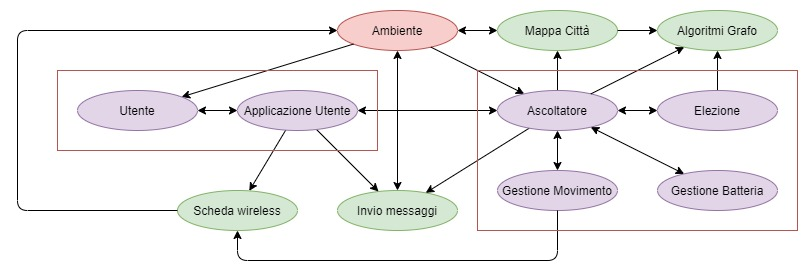
\includegraphics[width=15cm]{schema_moduli_livello_2.jpg}
	\caption{Dipendenza tra moduli e automi}
	\label{fig:schema_moduli_livello_2}
\end{figure}

Gli automi sono presenti nell'appendice.

L'immagine \ref{fig:automa_utente} rappresenta l'automa\_utente.

L'automa app\_utente è stato suddiviso, graficamente, in 2 automi : l'immagine \ref{fig:automa_app_utente_flusso}  rappresenta il flusso del semplice spostamento dell'utente, mentre l'immagine \ref{fig:automa_app_utente_stati} contiene tutti gli altri eventi che si possono ricevere nel mentre: cambiamento topologia, incidenti etc.

L'immagine \ref{fig:automa_moving} rappresenta l'automa\_moving.

L'immagine \ref{fig:automa_elezione} rappresenta l'automa\_elezione.

L'immagine \ref{fig:automa_batteria} rappresenta l'automa\_batteria.

L'immagine \ref{fig:automa_listener} rappresenta l'automa\_listener.

L'immagine \ref{fig:automi_macchina_various} rappresenta alcuni eventi globali per i taxi, ossia che interessano più stati di automi diversi.

\section{Protocolli e algoritmi}
In questa sezione vengono discusse le comunicazioni tra le diverse componenti e gli algoritmi utilizzati all'interno del sistema.

\subsection{Funzioni di costo delle macchine} \label{funzioni_di_costo_macchine}
Per la scelta della macchina più adatta, vengono considerati i seguenti parametri.

\begin{itemize}
	\item Crdt = Carica Rimanente Dopo Trasporto dell'utente.
	\item Cc = Costo Cliente, esprime dopo quanto tempo la macchina raggiungerebbe il cliente.
	\item Cr = Carica Rimanente espressa in unità di misura della distanza percorribile.
	\item Prc = Percorso Rimanente Cliente espresso in unità di misura della distanza assumendo che il taxi sia occupato.
	\item Pvcn = Percorso Verso Cliente Nuovo a partire dalla posizione dopo lo scorso cliente espresso in unità di misura della distanza.
	\item Pvdc = Percorso Verso Destinazione Cliente a partire dalla posizione attuale del cliente espresso in unità di misura della distanza.
	\item Pvcr = Percorso Verso Colonnina Ricarica per permettere alla macchina di ricaricarsi dopo il trasporto se necessario.
\end{itemize}

\begin{equation} \label{funzione_costo_raggiungimento_cliente}
Cc = Prc + Pvcn
\end{equation}

\begin{equation} \label{carica_rimanente_trasporto}
Crdt = Cr - (Cc + Pvdc + Pvcr)
\end{equation}

La scelta della macchina, verrà effettuata minimizzando il tempo del cliente \ref{funzione_costo_raggiungimento_cliente} e, in caso di parità, massimizzando la carica rimanente dopo il trasporto \ref{carica_rimanente_trasporto}. Nel caso in cui non sia univoco il vincitore, la selezione diventa casuale tra i contendenti.

\subsection{Pacchetti scambiati per l'elezione}\label{descrizione_pacchetto}
Vengono utilizzati tre tipi di pacchetti per l'algoritmo di elezione:
\begin{itemize}
	\item Inizio algoritmo elezione
	\item Risultati dei calcoli
	\item Notifica Vincitore
\end{itemize}

\subsubsection{Inizio algoritmo}
Lo scopo di questo pacchetto è di notificare ai nodi raggiungibili dal nodo corrente l'inizio dell'elezione. Esso è formato in questo modo:

\begin{lstlisting}
[ID_self, begin_election, Position_From, Position_To, TTL]
\end{lstlisting}

\begin{itemize}
	\item ID\_self: il riferimento a sé stesso per permettere l'impostazione del genitore agli altri nodi raggiunti.
	\item Position\_From: Posizione di partenza del percorso da calcolare.
	\item Position\_To: Posizione di arrivo del percorso da calcolare.
	\item TTL: Per evitare di dover visitare tutto il grafo delle comunicazioni tra le macchine, si è scelto di impostare un TTL al pacchetto affiché dopo un certo numero fisso di salti ci si fermi. Questo porta al fatto che non è garantito che la soluzione trovata sia quella ottimale, tuttavia ciò permette un compromesso tra una buona soluzione e una limitazione della possibile congestione dei messaggi. Inoltre permette una riduzione dei possbili conflitti tra diverse leader election.
\end{itemize}

Il sistema si aspetta che alla ricezione di questo messaggio, il nodo risponda con una notifica di acknowledgment, in tal modo il nodo inviante è sicuro che esso sia stato ricevuto.

\subsubsection{Risultato dei calcoli} \label{pacchetto_calcolato}
Questo pacchetto contiene i dati calcolati dai nodi raggiunti dal pacchetto "inizio algoritmo" assieme a quelli del nodo corrente. Esso verrà poi inviato al genitore e sempre tramite esso è possibile creare la tabella di routing dei nodi coinvolti nell'elezione. Tuttavia per la comunicazione del vincitore, non verrà utilizzata la suddetta tabella poiché è più efficiente effettuare un multicast.

\begin{lstlisting} 
[{ID_1, Cc_1, Crdt_1}, ..., {ID_N, Cc_N, Crdt_N}]
\end{lstlisting}

Esso contiene, in ordine, per ogni nodo i: 
\begin{itemize}
	\item ID\_i: riferimento al veicolo i.
	\item Cc\_i, Crdt\_i: i costi della macchina i come descritto nella funzione di costo \ref{funzioni_di_costo_macchine}
\end{itemize}

\subsubsection{Notifica Vincitore}\label{pacchetto_vincitore}
Scopo del pacchetto è di notificare il vincitore dell'elezione e rilasciare i nodi coinvolti in essa. Questo pacchetto è formato nel seguente modo:

\begin{lstlisting}
[ID_WINNER, ID_USER, winner]
\end{lstlisting}

Il nodo iniziatore lo crea e lo invia in multicast a tutti i nodi coinvolti nell'elezione. Il vincitore, ricevendolo, aggiorna la propria coda e notifica la presa in carico al cliente.

\subsection{Creazione dello Spanning Tree}

Per l'elezione è necessaria la creazione di uno Spanning Tree dei nodi partecipanti ad essa per le comunicazioni. L'Echo algoritm che viene utilizzato ne permette la creazione man mano che i nodi ricevono i messaggi di inizio elezione.

Ogni nodo che partecipa riceve dal genitore padre la notifica di inizio elezione e in tal modo viene creata una relazione padre-figlio tramite la quale possono comunicare. Se un nodo riceve lo stesso tipo di notifica ma possiede già un padre, risponde al mittente di non poter partecipare e non inoltra ai propri vicini la notifica.

La radice dello spanning tree è il nodo iniziatore.

\subsection{Algoritmo di Elezione}

Come già accennato nell'introduzione al punto \ref{intro_algo}, l'algoritmo di elezione scelto è di tipo Wave e ne soddisfa le notorie proprietà. In particolare, si è optato per un Echo algoritm poichè il grafo su cui deve essere applicato è indiretto ed è possibile che siano presenti dei cicli.
L'algoritmo segue i seguenti passi:

\begin{enumerate}
	\item La macchina iniziatrice, la quale viene scelta perché la più vicina al cliente oppure in seguito a degli eventi di aggiornamento della mappa o incidente, inizia la wave creando un pacchetto da inviare ai propri vicini formato come già descritto al punto \ref{descrizione_pacchetto}, poi calcola i propri costi come descritto nella parte \ref{funzioni_di_costo_macchine}, ed aspetta i dati dei nodi che hanno risposto in modo positivo con l'acknowledgment al pacchetto di inizio elezione.
	\item Ogni nodo che riceve il pacchetto di inizio elezione, se non sta già partecipando a un'altra elezione, si sposta nello stato relativo al calcolo del leader. In ogni caso, risponde al nodo inviante se partecipa oppure no all'elezione. In caso negativo, non inoltra il pacchetto di inizio elezione ricevuto ai suoi vicini. In caso positivo, invece, se il TTL è superiore a 0, ne riduce il valore di un'unità e lo inoltra ai propri vicini. Successivamente, come per il nodo padre, si mette in attesa degli ack dei vicini.
	\item Il nodo che riceve il pacchetto di starting election con TTL pari a zero, dopo avere inviato l'ack al genitore, non inoltra ulteriormente l'inizio dell'elezione ai vicini.
	\item Ogni nodo, dopo aver ricevuto l'ack da parte dei figli alla partecipazione dell'elezione, calcola i propri costi e si mette in attesa che i propri figli, se presenti, gli mandino i costi calcolati. Alla ricezione di tutti i costi dei figli esso crea un pacchetto unico concatenando i costi ricevuti al proprio. Successivamente inoltre il pacchetto risultate al padre. Per la struttura di esso si faccia riferimenti a \ref{pacchetto_calcolato}.
	\item Dopo aver inviato al padre i dati relativi ai costi, ogni nodo si mette in attesa di conoscere chi è il leader.
	\item Quando il nodo iniziatore riceve tutti i dati calcola il leader in base alle proprietà descritte nella parte \ref{funzioni_di_costo_macchine}. Nel caso in cui non sia presente alcun vincitore, l'identificativo del miglior taxi viene impostato a un valore di errore.
	\item L'iniziatore invia il messaggio contenente il leader in multicasting a tutti i partecipanti all'elezione. Si faccia rifermento alla parte \ref{pacchetto_vincitore} per la descrizione del pacchetto.
	\item Tutti i nodi ricevono la notifica del leader e in base al risultato compiono le azioni più opportune. In ogni caso escono dallo stato di elezione eliminando tutte le informazioni calcolate.
	\item In base al vincitore si hanno due casistiche:
		\begin{itemize}
			\item Vincitore presente: il nodo corrispondente aggiorna la propria coda dei nodi da visitare e comunica al modulo di ricezione del cliente, tramite le celle di comunicazione descritte nell'introduzione al punto \ref{problematiche_distribuite}, di essere pronto a servirlo e se egli è in coda oppure no.
			\item Vincitore assente: il nodo iniziatore invia il pacchetto contenente l'id con errore anche all'applicazione dell'utente.
		\end{itemize}
\end{enumerate}

Un esempio dei pacchetti scambiati durate l'algoritmo è presente all'immagine \ref{fig:pacchetti_macchina_elezione}. La parte in basso a sinistra mostra lo spanning tree creato.

\begin{figure}[htbp]
	\centering
	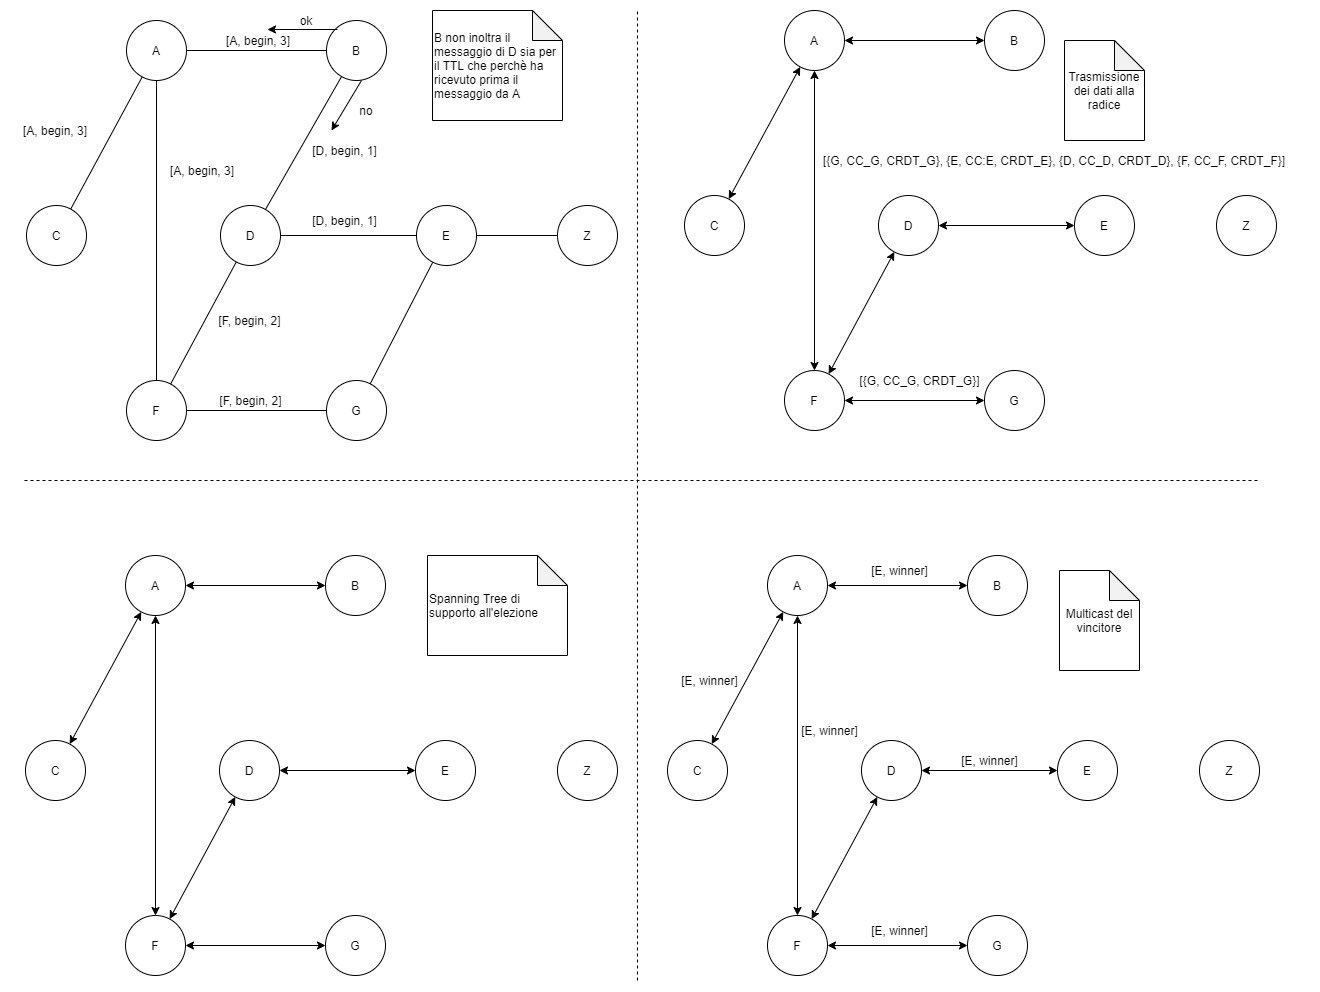
\includegraphics[width=14cm]{pacchetti_macchina_elezione.jpg}
	\caption{Rappresentazione dei messaggi scambiati durante l'elezione.}
	\label{fig:pacchetti_macchina_elezione}
\end{figure}

\newpage

\subsection{Possibili errori durante l'elezione}

I problemi durante l'esecuzione dell'algoritmo nel sistema sono i seguenti:
\begin{itemize}
	\item Aggiornamento della mappa.
\end{itemize}

I problemi possibili ma assenti per via dell'implementazione del sistema sono i seguenti:
\begin{itemize}
	\item Rimozione di una macchina
	\item Perdita di pacchetti
\end{itemize}

\subsubsection{Aggiornamento della mappa}
Viene discussa nella sezione Aggiornamento Mappa \ref{aggiornamento_mappa}.

\subsubsection{Rimozione di una macchina}
Sebbene il sistema venga costruito in modo che una vettura possa essere rimossa solamente se si trova nello stato ``idle'', è bene gestire i casi in cui l'eliminazione avvenga in ogni possibile stato, compresa l'elezione. Per risolvere il problema di attesa della risposta da un taxi ormai rimosso, ogni nodo invia dei messaggi di tipo ``hello'' per controllare lo stato della vettura di cui sta aspettando il calcolo dei costi. In tal modo se non ricevono risposta entro un tempo ragionevole lo considerano rimosso e continuano l'algoritmo di elezione.

\subsubsection{Perdita di pacchetti}
Nel caso in cui vengano persi dei pacchetti durante qualsiasi fase dell'elezione, è possibile accorgersene poiché vengono restituiti i messaggi di acknowledgment. Una soluzione per questo problema è l'utilizzo del protocollo TCP.

\subsection{Aggiornamento della mappa}\label{aggiornamento_mappa}

Questa casistica considera il caso in cui i percorsi calcolati, nel caso utilizzino degli archi deprecati, non siano più validi. 

L'aggiornamento può avvenire in diversi momenti e stati della macchina. 

\begin{itemize}
	\item Macchina in stato ``idle'': semplice aggiornamento, non comporta alcun problema.
	\item Macchina in stato ``Running Election'': l'automa ``ascoltatore'' si trova nello stato ``listen\_election'', quindi l'aggiornamento avviene non appena l'elezione si è conclusa.
	\item Macchina in stato ``Moving'': significa che la coda dei punti da visitare non è vuota. Nello stato ``update\_map'' dell'automa ``ascoltatore'' vengono calcolati quanti utenti presenti nella coda possono essere soddisfatti e quindi si hanno tre possibili scenari:
	\begin{itemize}
		\item Tutti i clienti sono soddisfatti: notifica ai clienti con i nuovi tempi di percorrenza.
		\item Alcuni clienti soddisfatti: i clienti soddisfatti ricevono un messaggio con i nuovi tempi, gli altri un messaggio di impossibilità nel soddisfare la richiesta. Sarà l'applicazione dell'utente a far ripartire l'elezione.
		\item Nessun cliente soddisfatti: tutti i clienti riceveranno la notifica di impossibilità di erogazione del servizio.
	\end{itemize}
\end{itemize}

\subsection{Diagrammi di sequenza dei messaggi}
All'appendice \ref{messaggi_scambiati_appendix}, sono presenti i diagrammi di sequenza dei messaggi che vengono scambiati tra i diversi moduli per permettere le funzionalità del sistema. Il modulo di comunicazione dei messaggi non viene incluso nei diagrammi poiché sottinteso ad ogni comunicazione. L'invocazione di questo modulo corrisponde, negli automi, al passaggio a un generico stato che inizia con ``send'', pertanto anche questi stati non vengono riportati.
I riquadri di colore giallo indicano gli stati mentre quelli di colore rosso indicano un riferimento ad altri diagrammi di sequenza.

Questi messaggi vengono scambiati durante il flusso normale del servizio, nel caso non siano presenti eventi problematici.
\begin{enumerate}	
	\item Richiesta da parte dell'utente del servizio di trasporto \ref{fig:messaggi_utente_request_car}.
	\item Messaggi scambiati dall'applicazione dell'utente per la richiesta di un taxi. Questa è l'elezione dal punto di vista dell'app. \ref{fig:messaggi_app_utente_elezione}. Nella rappresentazione sono stati inseriti due veicoli, un iniziatore e un vincitore. In base ai risultati dell'elezione il messaggio del vincitore viene inviato dall'entità adatta. Il riquadro rosso con all'interno la scritta ``Cars running Election'' fa rifermento al relativo diagramma dei messaggi, vale a dire al punto 3.
	\item Messaggi scambiati tra la macchina iniziatrice dell'elezione e le altre partecipanti. In questo grafico viene mostrato il flusso completo nel caso in cui non sorgano problemi durante l'elezione. \ref{fig:messaggi_macchina_iniziatore_elezione}. La macchina vincitrice, oltre ad aggiornare la coda dei punti da visitare, notifica all'utente il proprio riferimento e il tempo di attesa per esaudire la richiesta
	\item Movimento del taxi alla posizione dell'utente e successivo trasporto \ref{fig:messaggi_utente_trasporto}. In questa fase vengono consumati i punti contenuti nella coda dell'automa movimento del taxi. Ogni punto è etichettato e in base al tipo di punto viene inviato un messaggio all'utente.
\end{enumerate}

Questi sono i messaggi scambiati nella gestione dei possibili eventi gestiti dal sistema. Nel caso dell'utilizzo di variabili presenti in automi diversi dal proprietario, vengono utilizzati i messaggi definiti al primo punto. Nelle successive rappresentazioni, questa parte verrà omessa poiché le frecce punteranno direttamente all'automa destinatario.

Si assume che i messaggi interni alla macchina, quindi scambiati tra gli automi, giungano sempre a destinazione.

\begin{itemize}
	\item Messaggi scambiati dagli automi internamente alla macchina per il passaggio dei valori degli attributi. \ref{fig:messaggi_macchina_get_attribute}
	\item Messaggi scambiati tra gli automi nel caso in cui il livello della batteria scende sotto il minimo durante il viaggio della macchina. L'automa della batteria abilita il percorso verso la colonnina di ricarica. \ref{fig:messaggi_macchina_batteria}
	\item Messaggi scambiati tra gli automi nel caso in cui il livello della batteria resti costante per un tempo fissato. In tal caso si assume che la batteria venga ricaricata dai pannelli solari della macchina. \ref{fig:messaggi_macchina_pannelli_solari}
	\item Messaggi scambiati durante l'aggiornamento della mappa come già spiegato nella relativa parte \ref{aggiornamento_mappa}. \ref{fig:messaggi_macchina_update_map}
	\item Nel caso l'utente voglia cambiare destinazione, possono avvenire diversi scambi messaggi. \ref{fig:messaggi_utente_cambio_destinazione}
	\item Messaggi nel caso in cui avvenga un incidente. L'ambiente controlla che una macchia sia in movimento. \ref{fig:messaggi_macchina_incidente}
	\item L'ambiente sceglie un taxi tra quelli rotti e lo ripara. \ref{fig:messaggi_macchina_fixcar}
	\item L'ambiente decide quando rimuovere una macchina dalla mappa e per farlo invia un messaggio. \ref{fig:messaggi_macchina_rimozione}
\end{itemize}

\newpage

\section{Architettura fisica e Distribuzione} \label{arch_fisica}
Per l'implementazione fisica del progetto, è necessario che ogni automobile elettrica sia dotata di una scheda Wi-Fi per la comunicazione. Il cliente per poter usufruire del sistema necessita di utilizzare un'applicazione dedicata dal suo smartphone per le prenotazioni. Si suppone esista già la mappa della città nel formato adatto, ogni automobile ne deve possedere una copia nel disco locale. Un altro requisito hardware è che le macchine dispongano di sufficiente potenza computazionale per effettuare velocemente il calcolo dei percorsi. Si assume inoltre che sia già presente un'interfaccia che fornisca le primitive per lo spostamento della macchina: esse vengono utilizzate dall'automa movimento interno al modulo di gestione del taxi.

I moduli descritti nella sezione \ref{modules} sono associati ai componenti fisici in questo modo:
\begin{itemize}
	\item Il modulo utilizzato per la comunicazione da parte delle entità è composto da due parti: modulo ``localizzatore vicini'', dedito alla ricerca delle vicine entità, e modulo ``invio messaggi'', il cui scopo è controllare la buona formattazione dei dati da inviare e la spedizione stessa.
	\item Il modulo ``gestione tempo'', interno ad ogni entità del sistema, rappresenta l'orologio interno del dispositivo.
	\item Per quanto riguarda l'entità ``Utente'' descritta all'inizio del capitolo, l'omonimo modulo ne rappresenta un'astrazione e pertanto non possiede una controparte fisica. Il modulo ``interfaccia cliente-servizio'' corrisponde all'applicazione sullo smartphone dell'utente.
	\item I moduli ``mappa città'' e ``algoritmi grafo'' modellano il navigatore interno che permette l'accesso alla mappa precedentemente nominata e il calcolo dei percorsi.
	\item Il modulo ``gestione macchina'' contiene gli automi che permettono il funzionamento intelligente del taxi, come avverrebbe nel mondo reale.
	\item Il modulo ``elezione'' viene utilizzato dal corrispondente automa, pertanto non ha una controparte fisica.
\end{itemize}

\newpage

\section{Piano di Sviluppo}
% Since it is diffcult to predict just how hard implementing a new system will be, you should formulate as a set of "tiers", where the basic tier is something youre sure you can complete, and the additional tiers add more features, at both the application and the system level.

Sono stati individuati due insiemi di funzionalità che è necessario supportare.
\subsection{Funzionalità Base}

\begin{enumerate}
	\item Comunicazione peer to peer per la leader election.
	\item Richiesta dell'utente di trasporto.
	\item Gestione della ricarica delle macchine.
	\item Cambio di direzione di utente singolo.
	\item Gestione degli incidenti sia delle macchine che delle strade rotte.
\end{enumerate}

\subsection{Funzionalità Aggiuntive}

\begin{itemize}
	\item Perdita delle connessioni mentre si elegge il leader.
	\item Partecipazione della macchina già impegnata alla leader election.
	\item Possibilità di rimuovere la prenotazione
	\item Possibilità di cambiare destinazione anche se ci sono altri utenti nella coda della macchina candidata. Questa funzionalità vale per tutti gli utenti in coda, tuttavia è limitata dalla nuova destinazione che deve costare meno rispetto alla precedente.
	\item Car sharing fino a tre persone.
\end{itemize}

\subsection{Ordine di sviluppo}
Lo sviluppo dell'applicazione verrà suddiviso in diverse versioni via via estese con le nuove funzionalità. In particolare si seguirà questo ordine:

\begin{enumerate}
	\item Ogni macchina potrà parlare con tutte le altre macchine; l'utente invia la richiesta di trasporto alla macchina più vicina a lui; se un veicolo è impegnato con un cliente non partecipa alla selezione del leader per il trasporto ma fa da ponte per i vicini; la comunicazione tra i veicoli è diretta, quindi ogni taxi può parlare con chiunque.
	\item Vengono aggiunte le colonnine di ricarica, alle quali le macchine devono far rifornimento se stanno esaurendo le batterie; le macchine possono guastarsi; l'utente può decidere di cambiare destinazione.
	\item Rottura delle strade ma senza disconnessione del grafo stradale.
	\item Le macchine possono comunicare solo con quelle vicine.
	\item La macchina partecipa all'elezione anche se al momento è già impegnata, tuttavia si considera disponibile solo dopo aver compiuto il tragitto già attivo.
	\item Le connessioni tra le macchine possono perdere andare perse mentre si elegge il leader.
	\item Rimuovere prenotazione.
	\item Cambio direzione anche se in lista.
	\item Implementazione del car-sharing fino a 3 clienti.
\end{enumerate}